\graphicspath{{chapters/_resources/}}

\chapter{Telomeres and telomere transcription in cancer}

\hypertarget{what-are-telomeres}{%
\section{What are telomeres?}\label{what-are-telomeres}}

A DNA double strand break (DSB) generates new chromosome ends, which are
structurally similar to a telomere. But what is so special about the
extremities of our chromosomes?

Telomeric DNA is made of \emph{telomeric repeats}, 2-20kb in length and
forming GC rich sequences (seen when talking about R-loops). They depend
on the current cell cycle phase. A few nucleotides before telomeres we
find \emph{subtelomeric repeats} (''patchwork'' sequences duplicated
during evolution, devoid of genes and less conserved).

\textbf{Study from Barbara McClintock}: she treated chromosomes with
X-Rays and she observed large chromosomal aberrations, since breaks can
be repaired by the fusion among different chromosomes. However, she
noticed that such fusions never occurred between extremities. Somehow
the physiologic ends of chromosomes were protected from these fusions.
Even if chromosomes end with the exact same sequence, there are no
identical extremities, as the t-loop can invade in different positions.

\hypertarget{telomeres-mask-chromosome-ends-from-being-recognized-as-double-strand-breaks}{%
\section{Telomeres mask chromosome ends from being recognized as double-strand breaks}\label{telomeres-mask-chromosome-ends-from-being-recognized-as-double-strand-breaks}}

Telomeres form t-loops: mammalian telomeres end in a large loop. A
T-loop does not form by itself, but some proteins are involved. In
particular, TRF2 dimer facilitates the strand invasion - in fact
telomeres t-loops are TRF2 dependent.

Telomeric DNA is coated with telomere binding proteins → \emph{shelterin
complex} (Figure \ref{fig:shelt}). It contains: TRF1 and TRF2 (dsBP), POT1 (ssBP), RAP1, TIN2 and
TPP1 (bridging). The complex allows dsbp and ssbp to interact. We know
that there are also subcomplexes on telomeres.

\begin{figure}
\centering
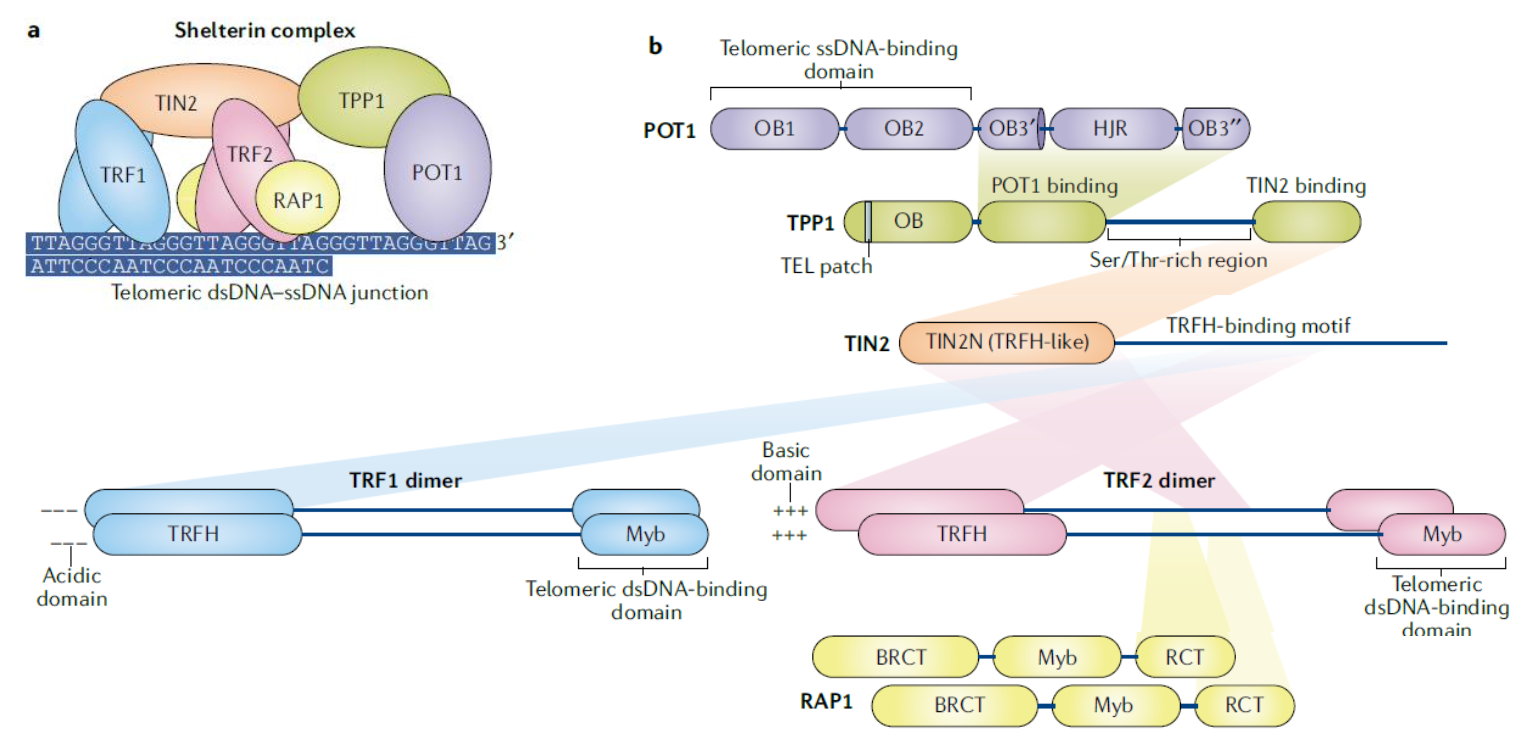
\includegraphics[width=0.5\textwidth]{../_resources/Screen_Shot_2022-12-15_at_17-43-24.png}
\caption{Lim and Cech, Nature Reviews Mol Cell Biol, 2021}
\label{fig:shelt}
\end{figure}

What is the function of this complex? Expression of a dominant negative
form of TRF2 (TRF2 B M), which is unable to bind telomeres, destabilizes
the shelterin complex. By removing the basic and main domain of the
stabilizing complex, the complex is disassembled. Telomere dysfunction
results in activation of DNA damage response at telomeres. Cells stop
dividing with this treatment, if the DDR pathway works correctly. The
impaired telomere structure induces DDR at chromosome ends leading to
dysfunctional telomeres.

TRF2 inhibits the recruitment of ATM through the formation of the t-loop
and then there's POT1, which represses the ATR pathway. POT1 can
displace RPA, which is not recruited and cannot interact with ssDNA.

\hypertarget{telomere-dysfunction-in-a-p53-and-rb-mutant-setting-does-not-induce-cell-cycle-block}{%
\section{Telomere dysfunction in a p53 and Rb mutant setting does not induce cell cycle block}\label{telomere-dysfunction-in-a-p53-and-rb-mutant-setting-does-not-induce-cell-cycle-block}}

Dysfunction of telomeres induces cell apoptosis through the usual P53-
and ATM dependent pathways. Problem: in cancer the apoptosis pathways
are often impaired.

IMR90 (Human Lung fibroblast), cell line HT1080 (sarcoma cell line) →
repress Cdk6, activate Cdk1. P53/Rb mutant cells continue dividing
despite the presence of dysfunctional telomeres ($\gamma$H2X).

Telomeres detected by DNA FISH on chromosome spread nicely co-localize
at chromosome ends in untreated IMR90 E6E7 cells. If we apply TRF2
depletion, we observe something different (Figure \ref{fig:ends}).

\begin{figure}
\centering
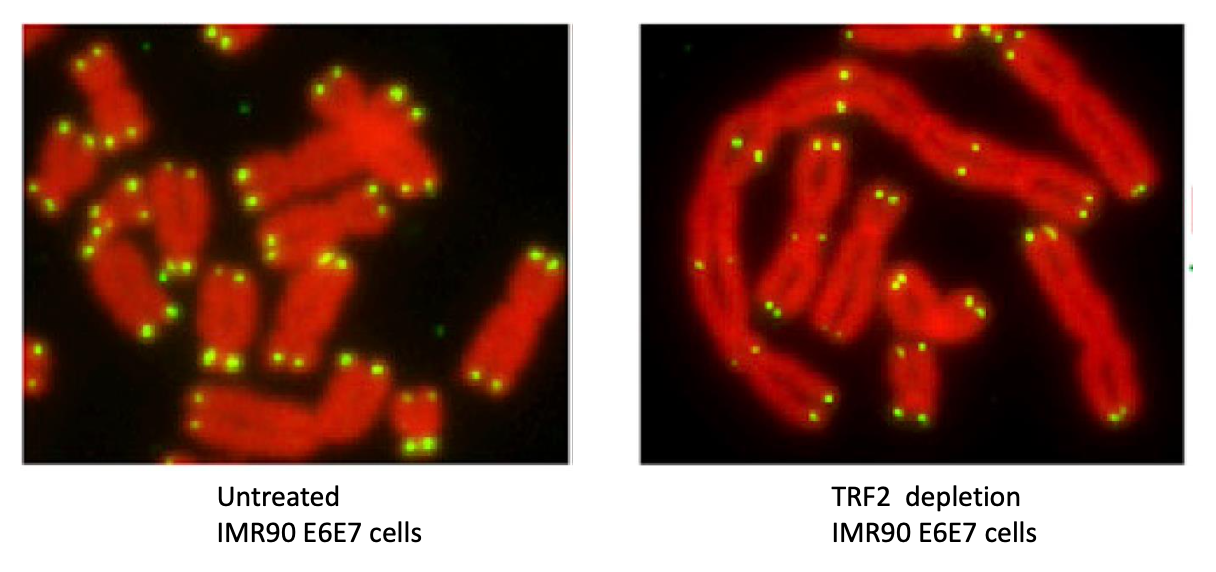
\includegraphics[width=0.5\textwidth]{../_resources/Screen_Shot_2022-12-15_at_17-54-31.png}
\caption{Cesare \emph{et al., Mol Cell} 2013}
\label{fig:ends}
\end{figure}

While the DNA damage response is not active, DNA repair pathways are
still active: cells continue proliferating and activating repair
mechanisms (in particular NHEJ) for what is perceived as a DSB. This
results in the fusion of chromosome ends → source of massive
\emph{genome instability}.

Dysfunctional telomeres in a p53/Rb mutant background associate with
genome instability.

\begin{figure}
\centering
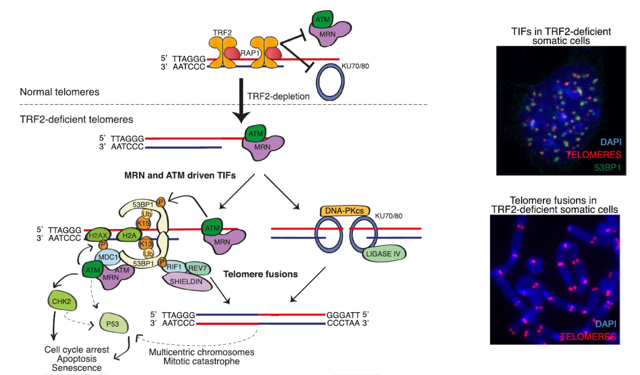
\includegraphics[width=0.5\textwidth]{../_resources/Screen_Shot_2022-12-15_at_17-49-51.png}
\caption{}
\end{figure}

The shelterin proteins inhibit DNA damage response and DNA repair
mechanisms at chromosome ends. By blocking shelterin
proteins, we reach \emph{senescence} (does not allow cell division,
incompatible with survival) or apoptosis, or chromosome fusions (Figure \ref{fig:bsh}).

\begin{figure}
\centering
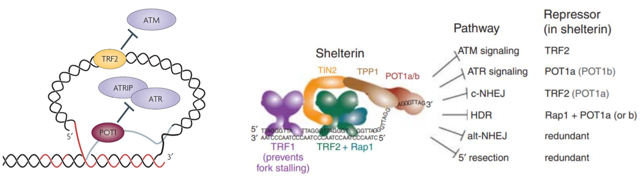
\includegraphics[width=0.5\textwidth]{../_resources/Screen_Shot_2022-12-15_at_17-49-02.png}
\caption{Doksani \& de Lange. \emph{Cold Spring Harbor Press.} 2014
Nature Reviews Cancer, 2008}
\label{fig:bsh}
\end{figure}

A few points to remember:

\begin{enumerate}
\def\labelenumi{\arabic{enumi}.}
\tightlist
\item
  Chromosome ends are capped by structures called telomeres
\item
  Telomeres are nucleoprotein complexes protecting the extremities of
  chromosomes from being recognized as DSBs (\textbf{The end protection
  problem})
\item
  Telomere function depends on the proper telomere structure and
  telomere binding proteins
\item
  Altered telomere structure leads to dysfunctional telomeres which are
  recognized as DSBs and trigger a DDR leading to senescence or
  apoptosis
\item
  If DDR pathway is impaired,  genome instability arises
\end{enumerate}

\hypertarget{end-of-replication-problem}{%
\section{End of replication problem}\label{end-of-replication-problem}}

``The end replication problem'' (eukaryotes have linear chromosomes) :
chromosome ends are not fully copied during DNA replication . Also, the
5' end is shorter than the lagging strand (because the template is
short). In addition, in the lagging strand, the RNA primers do not
anneal exactly at the last nucleosome, leading to uncertainty.

\begin{figure}
\centering
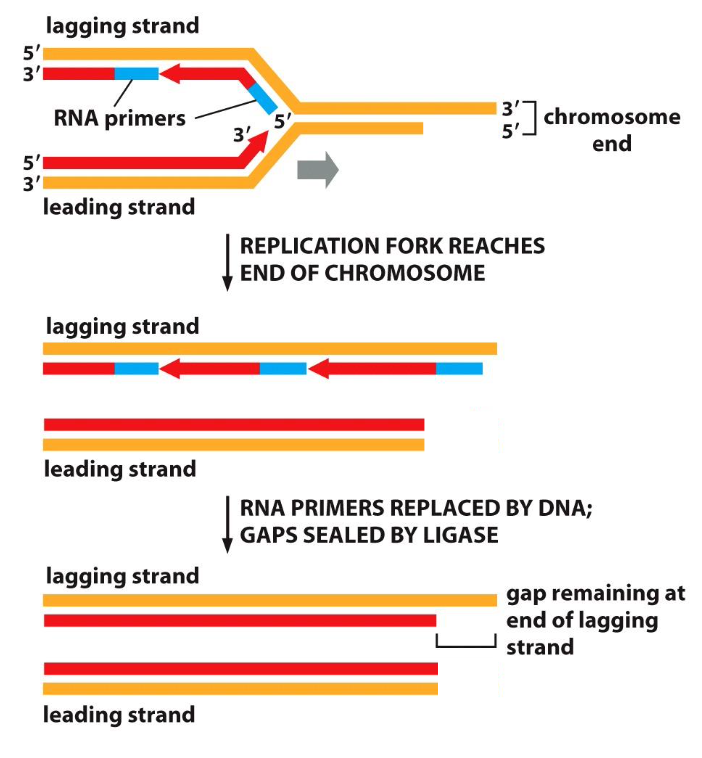
\includegraphics[width=0.5\textwidth]{../_resources/Screen_Shot_2022-12-15_at_18-00-30.png}
\caption{}
\end{figure}

Chromosome ends shorten at every cell division: the souther it
replicates, the shorter the chromosome end will become, due to an
intrinsic limitation of the DNA replication machinery.

Experimentally, we can check telomere length with:
\begin{itemize}
\tightlist
\item
  \textbf{Southern blot} analyses: genomic DNA is digested with capping
  enzymes, which do not cut inside telomeric repeats → full length
  telomeric sequences. Due to the fact that they are repetitive and
  replication is not complete, the first thing that we can observe is
  that telomere lengths are heterogenous, every telomere has a different
  length (stochastic).
\item
  \textbf{DNA-FISH}: usage of fluorescent probes binding in a sequence
  specific manner, the intensity of the signal is proportional on the
  quantity. The technique is usually applied during metaphase. If we
  were to do this on a population of fibroblasts, we could appreciate
  also the fact that different cells have different telomeres lengths.
\end{itemize}

\textbf{Telomere repeats are lost with age in human leukocytes}: we are
born with a pool of telomeres of a specific size, which will shorten
over time. But the shortening is not linear: 0-1 shortening of 400-500
hundred of bases per year and slows down. The shortening rates are not
even the same for every cell. There's also a sex bias: females have on
average longer telomeres both at birth and throughout life.

Telomeres shorten at each replication cycle up until a threshold, when
DNA breaks are introduced. In human stem cells, this results in a low
self-renewal capacity.

\hypertarget{hayflick-limit}{%
\subsection{Hayflick limit}\label{hayflick-limit}}

Discovery by Hayflick in 1961 (Hayflick limit): after a logarithmic
growth, cells reach a plateau. There exists a limited population number
that human cells can go through. The experiment involved fetal stem
cells, with lung cells being the best ones at diving. Inverse
correlation of age of the donor with max population doubling was
observed. \textbf{Telomere shortening associates with decreased
proliferative capacity of cells.}
\begin{itemize}
\tightlist
\item
  Telomere length correlates with the proliferative capacity of cells =
  our biological clock.
\item
  Cells with short telomeres enter senescence earlier than cells with
  longer telomeres.
\end{itemize}

Subsequent ChIP-on-chip experiments confirmed the presence of DNA damage
at the ends of chromosomes in senescent cells. Also, by removing
repairing pathways, it was found that cell cycle arrest in senescent
cells depends on DNA damage response pathways.

\hypertarget{triggering-senescence}{%
\subsection{Triggering senescence}\label{triggering-senescence}}

It's not actually the length of the telomeres that induces
\emph{senescence}, but their \emph{structure}. If we find a way to
promote t-loop formation, we can postpone senescence.

Study: TRF2 increased expression on telomeres promotes telomeres
shortening with a higher shortening rate - probably because of a more
stable t-loop, which impairs replication. Since telomeres are shorter,
we expect that they enter early senescence, but this is not observed →
senescence entrance does not depend on telomere length. It is the
altered structure triggering the activation.

Somatic cells will normally grow and reach the Hayflick limit,
triggering senescence. However, if we remove p53/Rb, we reach a M2
crisis, with increased genetic instability. The cells cannot sustain so
much genome instability, so they die because of the crisis. Replicative
senescence and crisis are two proliferative barriers controlled by
telomere deprotection.

It is thought that there are intermediate states of telomere length,
long enough to activate DNA damage response (sensed by cells) but not to
fusion (not short enough to cause disruptive events, uncapped).
Intermediate states are still kind of able to recruit the sheltering
complex.

\begin{figure}
\centering
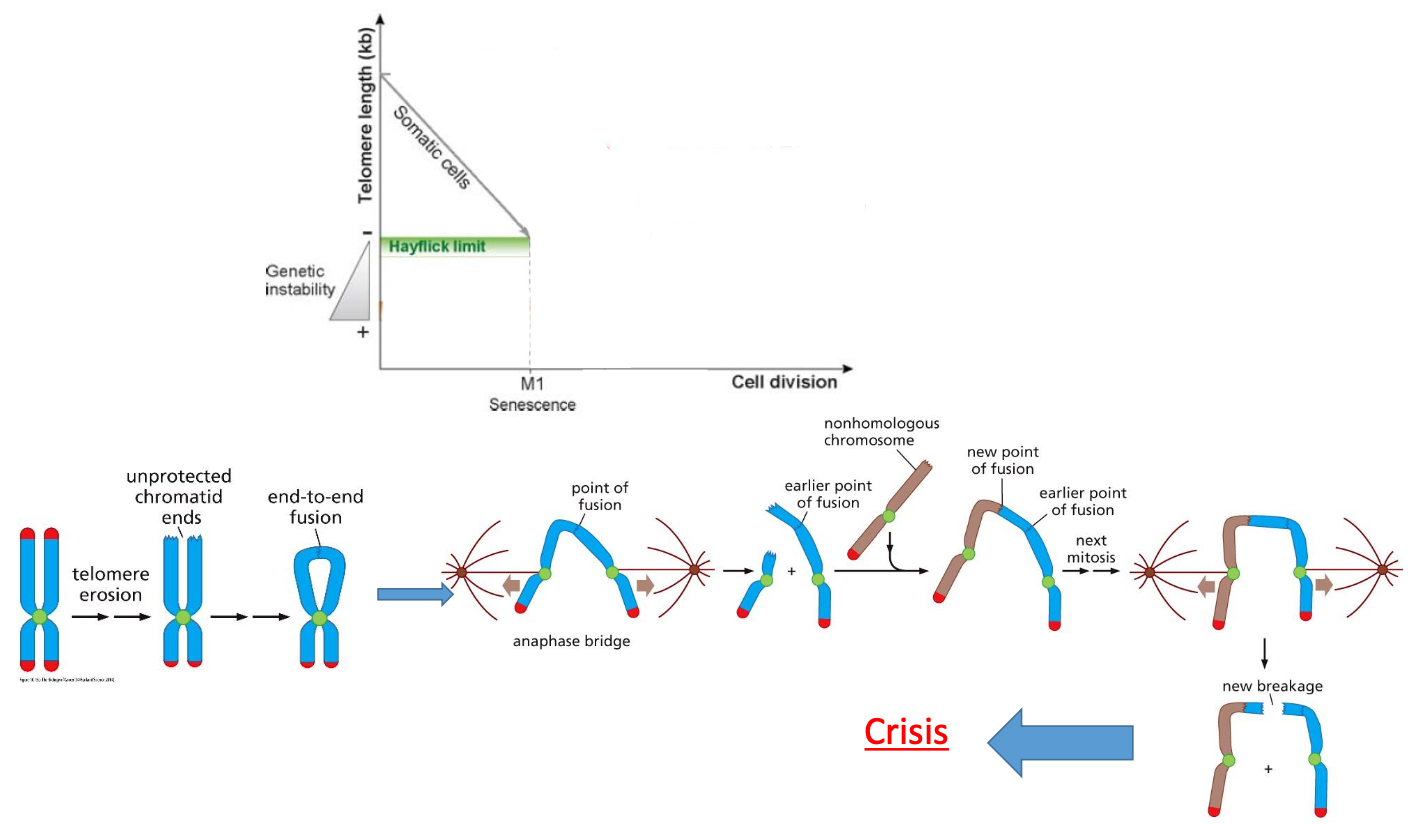
\includegraphics[width=0.5\textwidth]{../_resources/Screen_Shot_2022-12-15_at_22-39-00.png}
\caption{Stewart \& Weinberg. Ann Rev Cell Dev Biol, 2006}
\label{fig:crisis}
\end{figure}

Replicative senescence and crisis are independent cellular programs
induced by distinct telomere states and associated with distinct
biological outcomes.

\hypertarget{cell-crisis}{%
\section{Cell crisis}\label{cell-crisis}}

It is not yet clear how a cell crisis occurs (no p53 dependent death).
When cells approach crisis, by bypassing senescence, the time of mitosis
is extremely elongated: \emph{mitotic arrest} (from 30mins to hours).

During the \textbf{mitotic arrest,} we are at the spindle assembly
checkpoint, chromosomes are not properly attached by the two opposite
spindles. Due to the genomic instability provoked by short telomeres,
mitotic arrest amplifies telomeric deprotection, fostering the crisis (Figure \ref{fig:crisis}).

The way in which cells die is only now being discovered: during the prolonged
mitotic arrest exposed DNA activates DNA sensing mechanisms, triggering
a particular kind of \textbf{autophagic cell death}. Telomeric DNA
damage generates cytosolic DNA species with a fragile nuclear envelopes
that undergo spontaneous disruption. The cytosolic chromatin fragments
activate the cGAS-STING pathway and engage the autophagy machinery,
which is an integral component of the tumor suppressive crisis
mechanism.

\hypertarget{telomerase-enzyme}{%
\section{Telomerase enzyme}\label{telomerase-enzyme}}

Stem cells need to undergo hundreds of cell divisions without stressing
out. How can they do it?

In 1995, Greider and Blackburn managed to identify a specific telomere
terminal transferase activity in Teatrahymena (thermophile). In
thermophiles, there are a lot of very little chromosomes, with many
telomeres. When they incubated oligonucleotides with the sequence of the
telomeres, they observed elongation. An enzyme goes and duplicates it
also adding six more nucleotides. This could not be done with a regular
RNA polymerase, there is no template: the enzyme is perceiving and
elongating the sequence.

They found out that there exists an enzyme which also provides for the
template (Figure \ref{fig:temp}).

\begin{figure}
\centering
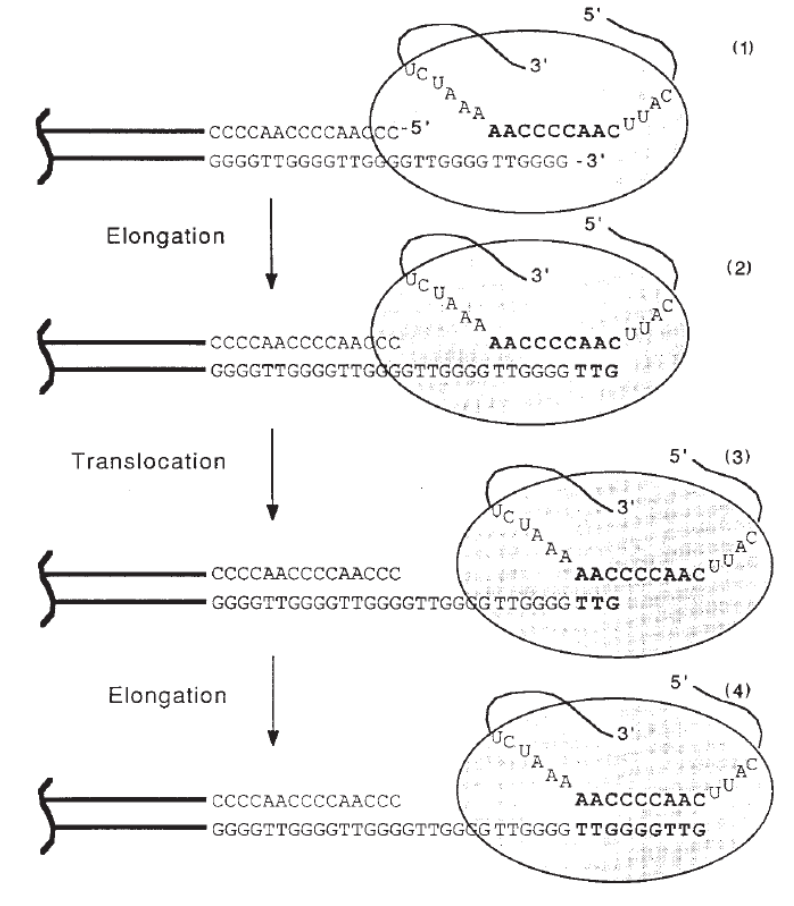
\includegraphics[width=0.4\textwidth]{../_resources/Screen_Shot_2022-12-15_at_22-58-03.png}
\caption{}
\label{fig:temp}
\end{figure}

In addition to the shelterin complex, also telomerase enzyme is
recruited on telomeric DNA (Figure \ref{fig:recr}). The telomerase RNA (TR) acts as a scaffold
module for telomerase assembly. The template is 11 bases long. The RNA
feature the presence of H-box domain, aiding in the recruitment of
TCAB1.

\begin{figure}
\centering
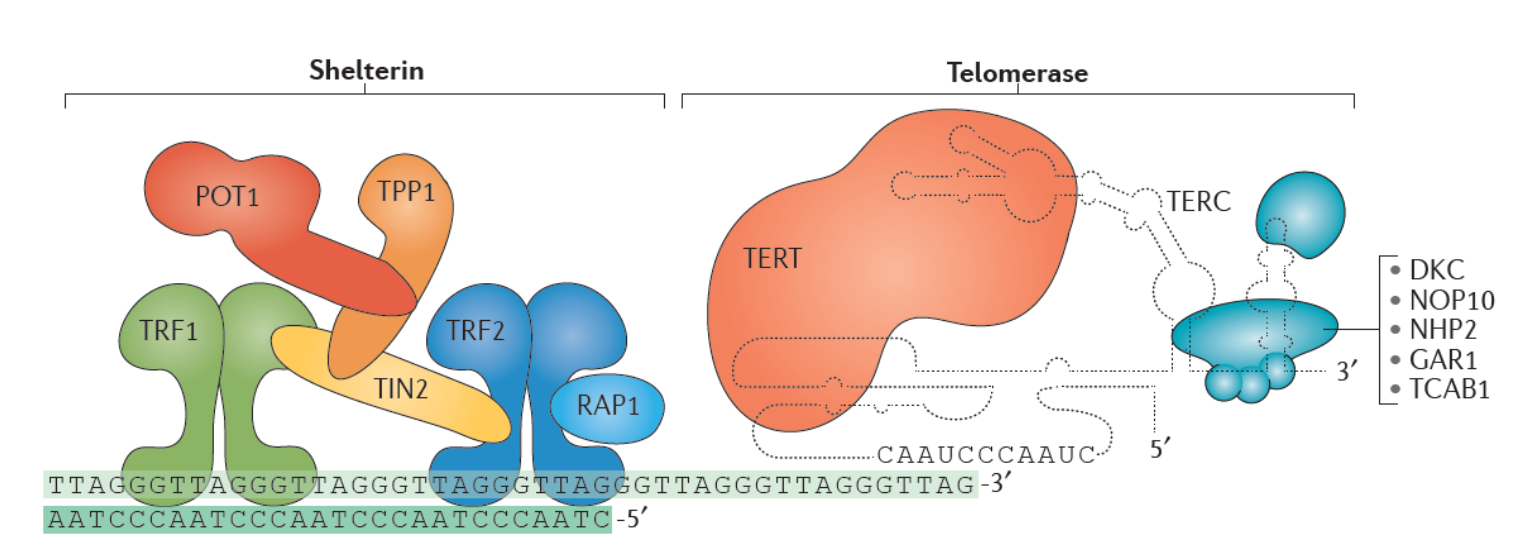
\includegraphics[width=0.5\textwidth]{../_resources/Screen_Shot_2022-12-15_at_22-58-28.png}
\caption{}
\label{fig:recr}
\end{figure}

Just after birth, telomerase activity drops. Some telomerase activity
can only be found in germ cell production (testicles). Telomerase
elongates telomeres in a stepwise manner, processive enzyme. Once it is
recruited, it is able to add 6-mers (not only 6 nts).

We also need to generate the second strand of telomeric DNA, since the
shelterin complex is recruited on dbDNA. Almost all eukaryotes use
telomerase to elongate telomeres.

\hypertarget{usage-of-telomerase}{%
\subsection{Usage of telomerase}\label{usage-of-telomerase}}

``Creation of human tumor cells with defined genetic elements'':
overexpressed hTERT to make up for telomere shortening, immortalization
(inhibition of p53 and Rb).

Mutations in TERT promoter represent the most frequent noncoding
mutations in cancer.


Shelterin proteins have two main functions:

\begin{enumerate}
\def\labelenumi{\arabic{enumi}.}
\tightlist
\item
  inhibit the activation of DNA damage response and DNA repair
  mechanisms
\item
  allow the recruitment of the telomerase enzyme
\end{enumerate}

Question by the audience: ``The overexpression of TRF2 and t-loop
formation inhibits replication. How is this achieved?''

It is presumed that the t-loop needs to be resolved in order to allow
RNA pol II access. Replication starts within subtelomeric regions and
moves towards chromosome ends. Under physiological conditions, the
t-loop is resolved. If we force TRF2 expression and t-loop formation, we
hinder transcription.

We highlighted the fact that chromosome ends shorten at every cell
division and at a certain point critically short telomeres have a
reduced amount of shelterin → unprotected, activation of DDR. Critically
short telomeres cannot fold into a functional structure due to the
paucity of bound shelterin complexes, trigger a DDR \& cell cycle arrest
leading to \emph{replicative senescence}.

Telomere-driven crisis and telomerase expression represent a crucial
path to genome instability. Cells can overcome crisis by activating
telomere maintenance mechanisms. Once the enzymes have been assembled at
chromosome ends, the long non coding Telomerase RNA acts as scaffold.
The recruitment of the enzyme is mediated by TP51???. Telomerase
selectively recognizes short telomeres.

The end replication problem also occurs in stem cells, but telomerase
comes to the rescue. In our normal cells telomerase is not there, the
catalytic subunit is silenced through epigenetic mechanisms. If we
overexpress TERT, telomerase activity can be established. The end
replication problem is actually good for us, it acts as a tumor
suppressing mechanism.

In the absence of p53 and Rb, we have another tumor suppressing
mechanism: if mutations hit TERT promoter, we are re-expressing
telomerase and healing the short telomeres. \textbf{Cells can overcome
crisis by activating telomere maintenance mechanisms.}

Mutations in TERT promoter represent the most frequent noncoding
mutations in cancer. The mutations are typically heterozygous, occur in
a mutually exclusive fashion, and both create an identical 11 bp
sequence `'CCCGGAAGGGG'. Telomerases are activated in cancer mainly by
two mutations in the promoter region, 146 and 124 C\textgreater T,
mutually exclusive. The mutation generates a new binding site for a TF,
GABPA, which acts as a dimer and allows long range chromatin
interactions.

\begin{figure}
\centering
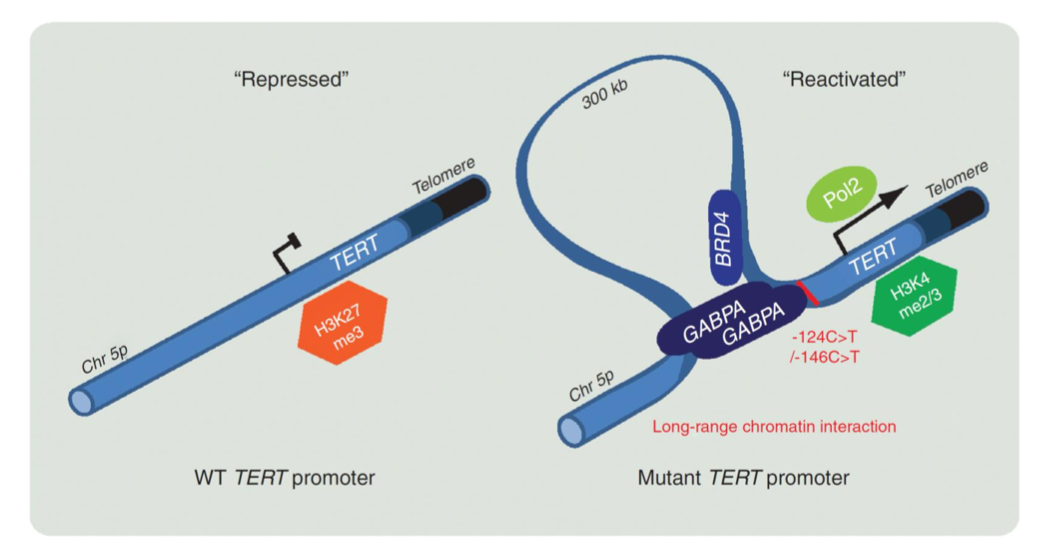
\includegraphics[width=0.5\textwidth]{../_resources/Screen_Shot_2022-12-17_at_17-53-38.png}
\caption{Min and Shay, \emph{Cancer Discovery} 2016}
\end{figure}

Also genomic abnormalities can activate TERT e.g.~close to activated
enhancer → hypermethylation, particularly true for neuroblastoma.
Therefore, telomerase represents an ideal target for cancer treatment.
During the years, it has been seen that the inhibition of TERT activity
(introduction of DN-hTERT) leads to cell death. It has been observed
that cancer cells have shorter telomeres although they are stable; this
could be due to the fact that telomerase is a rate limiting factor.
\emph{Imetelstat} is a first-in-class telomerase inhibitor which was
used in clinical trials, but had some side effects.

\hypertarget{alt}{%
\subsubsection{ALT}\label{alt}}

Cancer cells can develop resistance to telomerase-targeting therapies by
activating mechanisms of \emph{alternative lengthening of telomeres}
(ALT). This mechanism is quite complex, more mutations are required with
respect to telomerase activation.

\begin{figure}
\centering
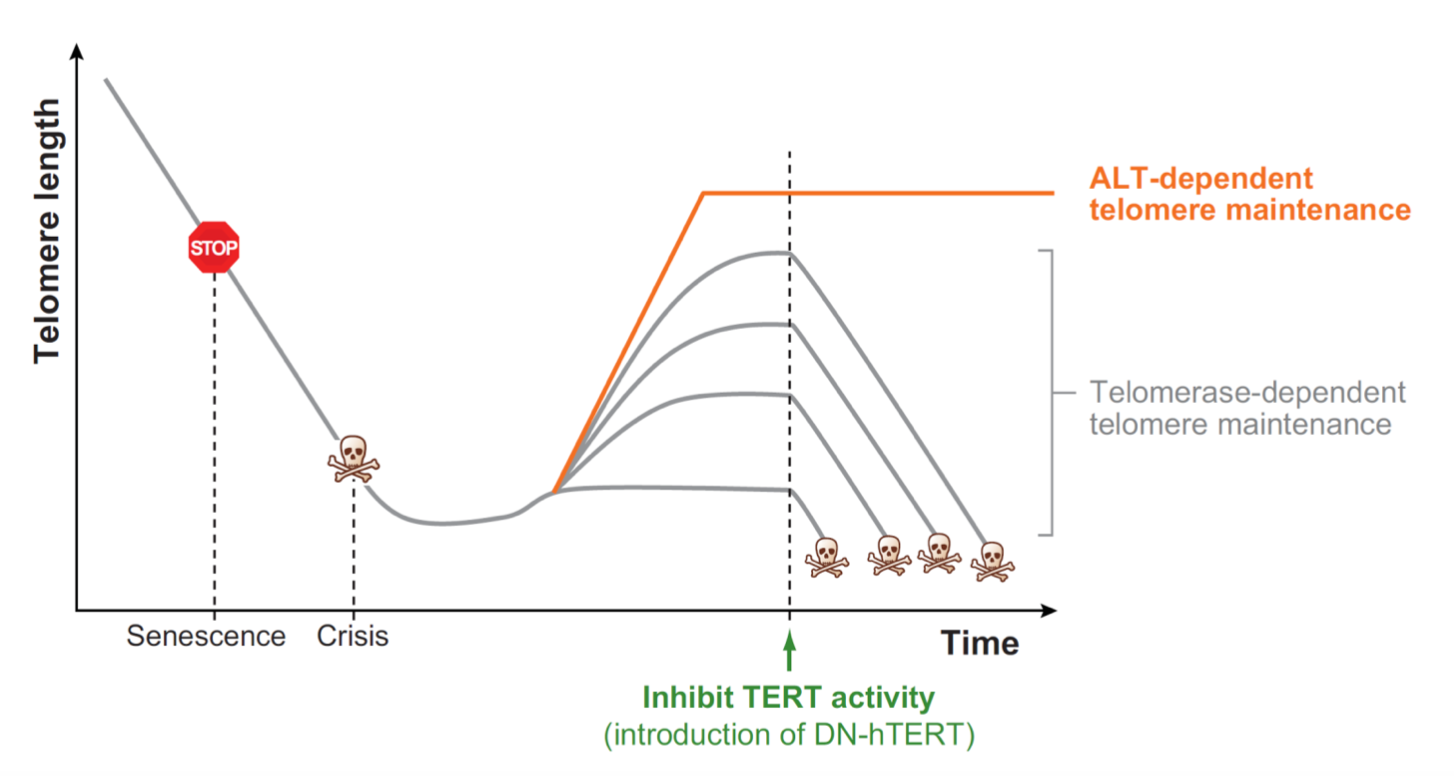
\includegraphics[width=0.5\textwidth]{../_resources/Screen_Shot_2022-12-17_at_17-44-43.png}
\caption{Screen Shot 2022-12-17 at 17-44-43.png}
\end{figure}

Alternative telomere lengthening mechanisms \textbf{(ALT) }rely on
homologous recombination among telomeres.

\begin{figure}
\centering
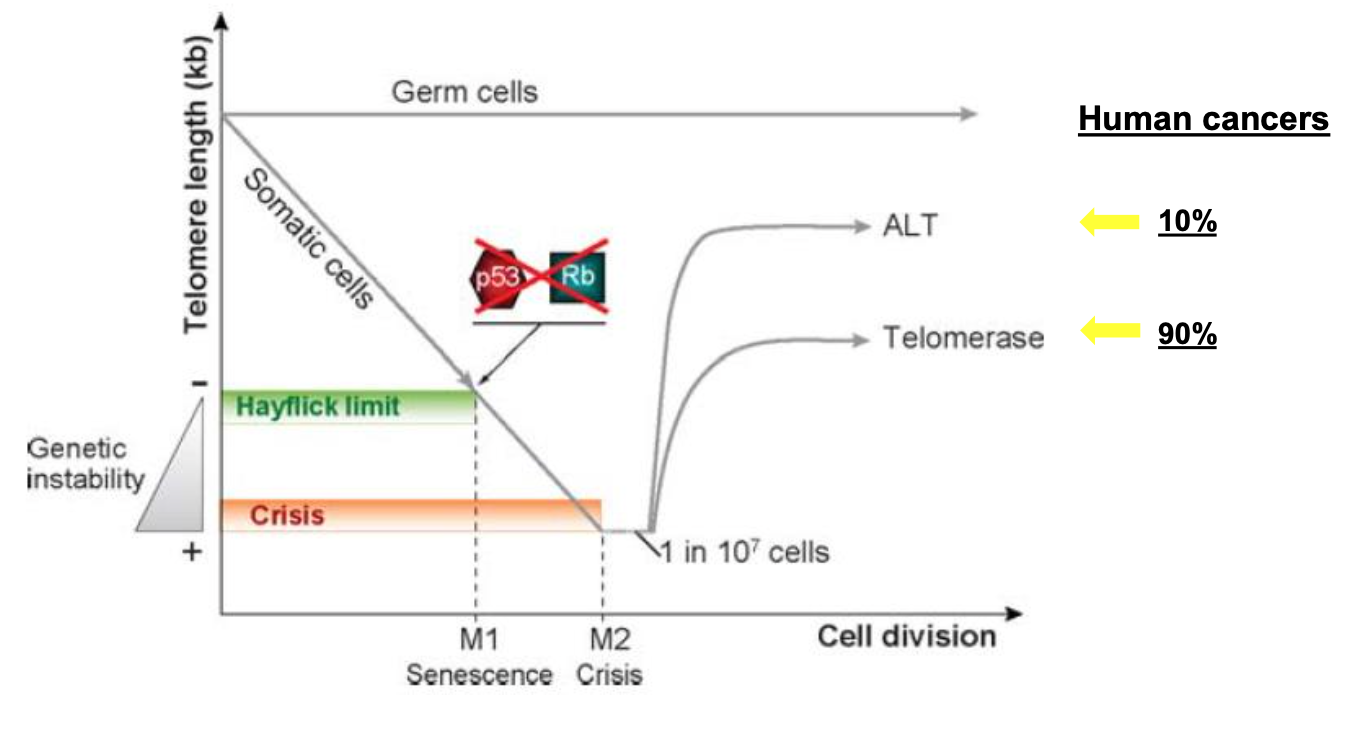
\includegraphics[width=0.5\textwidth]{../_resources/Screen_Shot_2022-12-17_at_18-04-37.png}
\caption{Screen Shot 2022-12-17 at 18-04-37.png}
\end{figure}

The 3' invades the sister chromatids, short telomere can prime DNA
replication → either the elongated strand goes back or nucleases cut and
we obtain an hybrid (exchange). Either way, the short telomere now
becomes long in the absence of telomerase (homologous recombination +
replication to finish the job). This process has some peculiarities with
respect to the telomerase mediated process:

\begin{itemize}
\item
  Telomeres have very heterogeneous length e.g.~reach up to 20 kB,
  invasion can occur anywhere in the telomeres, multiple invasions can
  occur\ldots{} No selection for the shortest telomere.
\item
  The process requires HR mediated mechanism (based on recombinases,
  \ldots). These enzymes are clustering in nuclear bodies containing
  promyelocytic leukaemia (PML) forming the so-called ALT-associated PML
  bodies (\textbf{APBs})
\item
  The product itself results in specific features: elevated rates of
  telomeric sister chromatid Exchanges (\textbf{TSCEs})
\item
  Abundant extra-chromosomal telomeric DNA in the form of
  double-stranded telomeric circles (t-circles), partially single
  stranded circles (\textbf{C- and G-circles}) and linear
  double-stranded DNA

  \begin{figure}
  \centering
  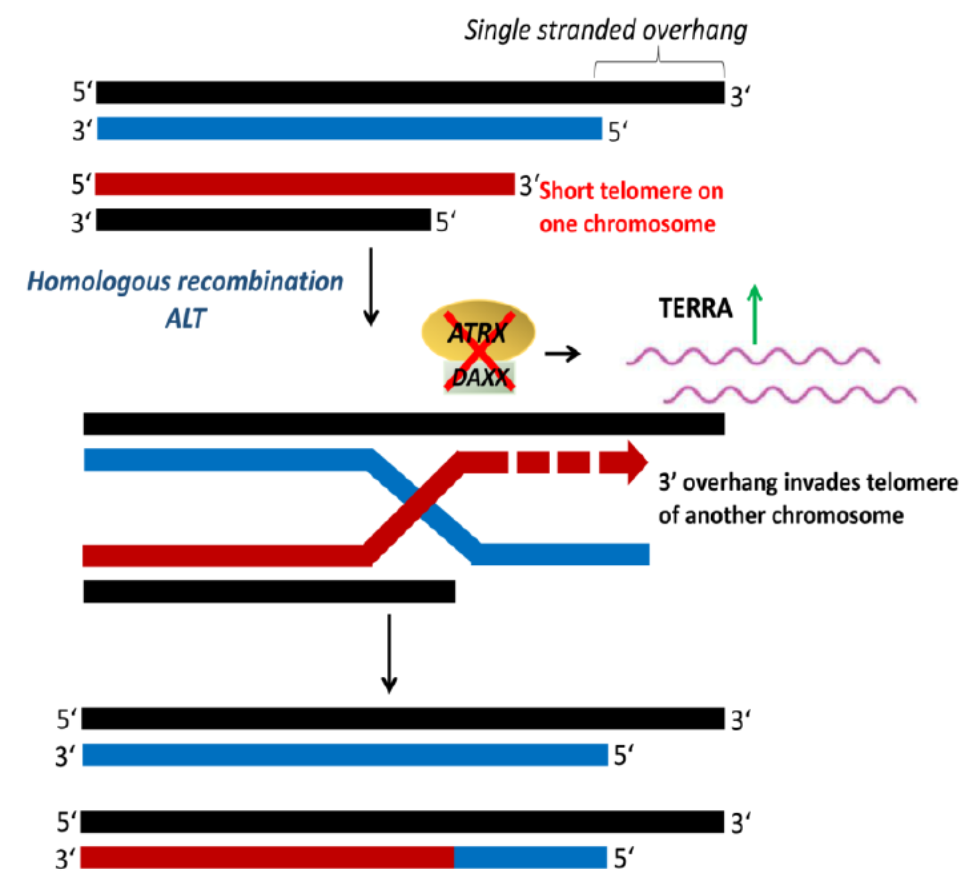
\includegraphics[width=0.5\textwidth]{../_resources/Screen_Shot_2022-12-16_at_21-36-20.png}
  \caption{Screen Shot 2022-12-16 at 21-36-20.png}
  \end{figure}
\end{itemize}

A key aspects in ALT tumors is the abundance of mutations in chromatin
remodeling complexes and histone chaperones. In addition, abundance of
long non coding RNA TERRA is becoming an additional marker for ALT
cancer cells.

\hypertarget{terra}{%
\subsection{TERRA}\label{terra}}

Telomeres are transcribed into \textbf{telomeric repeat-containing RNAs
TERRA}. Telomeres are transcribed in humans by RNA pol II and
polyadenylated. RNA pol II starts from 5' (subtelomeric region) and
proceed toward 3'. The sequences are G rich. A number of TF binding
sites have been identified and at least two types of promoters
regulating transcription:

\begin{itemize}
\tightlist
\item
  type-I promoter: very close to the telomeric repeat, within 1 kb
\item
  type-II promoter: up to 10kb distance from the telomeric repeat
\end{itemize}

We can identify distinct foci co-localizing with telomeres in several
organisms, TERRA expression is conserved in eukaryotes.

Several functions have been proposed and characterized for telomeric
transcripts. Key mechanism: promoting the recruitment of enzymes at the
chromosome ends. They interact with the shelterin complex and with a
plethora of proteins, including the origin of replication complex and
HP1. Transcripts localize to telomeres to regulate replication and
interact with TRF2, which could contribute to t-loop formation.

The transcript can engage in DNA hybrids. As we know, once an hybrid
forms the displaced strand is accessible to bp with telomeric
sequencing. R-loop formation fosters HR in ALT cancer cells and hinders
the advance of DNA polymerase → DNA replication stress and damage
response. The presence of R-loops can recruit TERRA factors. It is still
not clear whether these R-loops can only form in cis or also in trans.

In addition, telomeric transcripts not only localize at chromosome ends,
but also along the genome.

ChIRT technique: biotinylated probes after chromatin fixation. Instead
of using antibodies, we use TERRA probes. Thousands of binding sites
were detected in intergenic region, downregulation of TERRA leads to
altered gene expression.

Proposed TERRA functions:

\begin{itemize}
\tightlist
\item
  recruitment of enzymatic activities at chromosome ends
\item
  formation of DNA:RNA hybrids(R-loops) promoting HR among telomeres
\item
  regulation of gene expression
\item
  regulation of telomerase activity
\end{itemize}

TERRA is not detectable in WT cells by Northern blot; while mutating
cells, it was possible to observe a signal. RT-qPCR analyses showed some
TERRA signal in WT cells. Is it possible that in WT cells only a small
fraction of cells express TERRA at any given time?

A live cell imaging assay was set up to study TERRA from a single
telomere in living cells. MS2 system based on the fact that RNA is short
and interacts with the bacteriophage, if transcription is on MS2 will be
transcribed and signalled by GFP. It was seen that only a fraction of
cells express TERRA. But is this expression dependent on a particular
cell state?

\begin{figure}
\centering
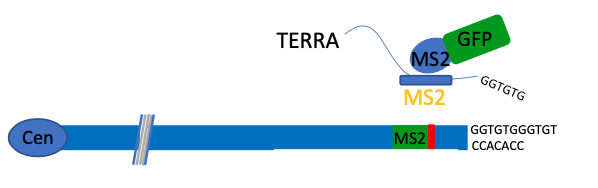
\includegraphics[width=0.5\textwidth]{../_resources/Screen_Shot_2022-12-16_at_21-50-07.png}
\caption{Screen Shot 2022-12-16 at 21-50-07.png}
\end{figure}

Using the MS2 and PP7 (two different bacteriophages) systems to analyze
TERRA expression from different telomeres in a same cell. TERRA
expression is controlled independently by each chromosome end, only a
little fraction shows co-expression of the two.

Generation of yeast strain containing an inducible short telomere 6R
(cassette). If we express recombinase we can remove the cassette and
obtain critically short telomeres (galactose). By leaving them grow,
there is not much of a difference in generation. The generation with
shortest telomeres are highest levels of TERRA. This suggests that there
is an in cis mechanism induced by short telomeres leading to TERRA
expression. TERRA levels are upregulated at short telomeres
(tlc1\(\Delta\) cells).

In order to investigate the function there are different approaches: we
can exploit imaging to detect the position of TERRA. Single acquisition
analyses indicate that Tel6R or Tel1L TERRA foci are not stably
associated with telomere 6R, no co-localization. If we instead use live
imaging, cells are monitored over time and we can obtain the dynamics.
TERRA molecules transiently colocalize with their telomere of origin.
But does it also colocalize with other telomeres?

TERRA focus preferentially co-localizes with its telomere of origin
during S phase in cis.

\begin{figure}
\centering
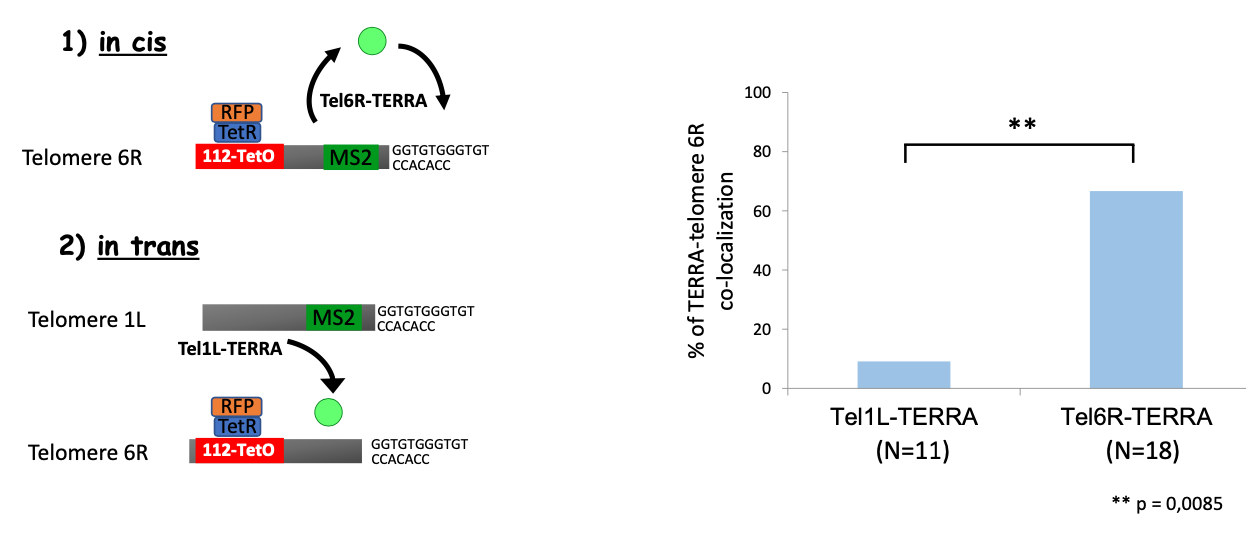
\includegraphics[width=0.5\textwidth]{../_resources/Screen_Shot_2022-12-17_at_11-01-12.png}
\caption{Screen Shot 2022-12-17 at 11-01-12.png}
\end{figure}

Telomerase elongates short telomeres during S phase → TERRA is recruited
at its telomere of origin during S phase, there could be an association
with telomerase. Indeed TERRA interacts with telomerase in vivo.

\begin{figure}
\centering
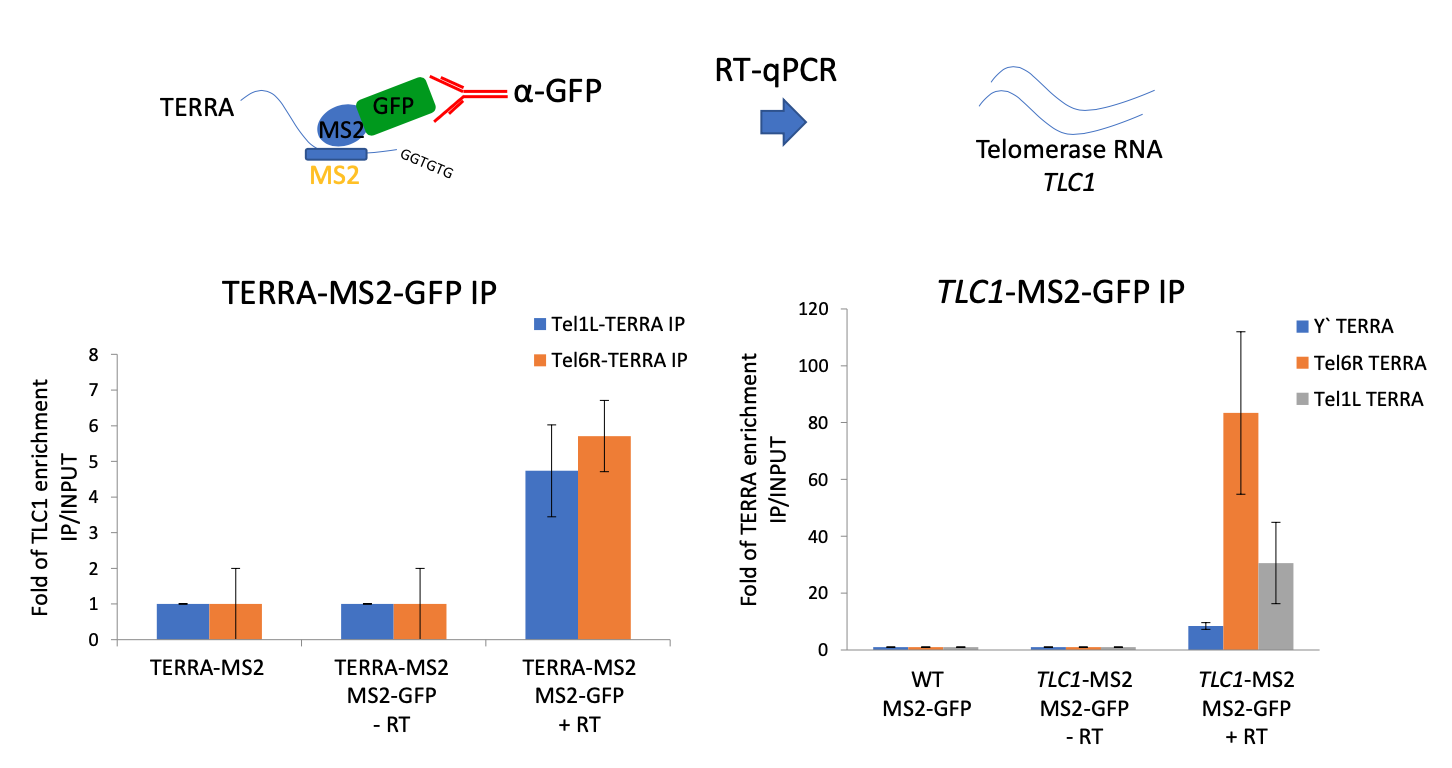
\includegraphics[width=0.5\textwidth]{../_resources/Screen_Shot_2022-12-17_at_11-02-44.png}
\caption{Screen Shot 2022-12-17 at 11-02-44.png}
\end{figure}

\begin{figure}
\centering
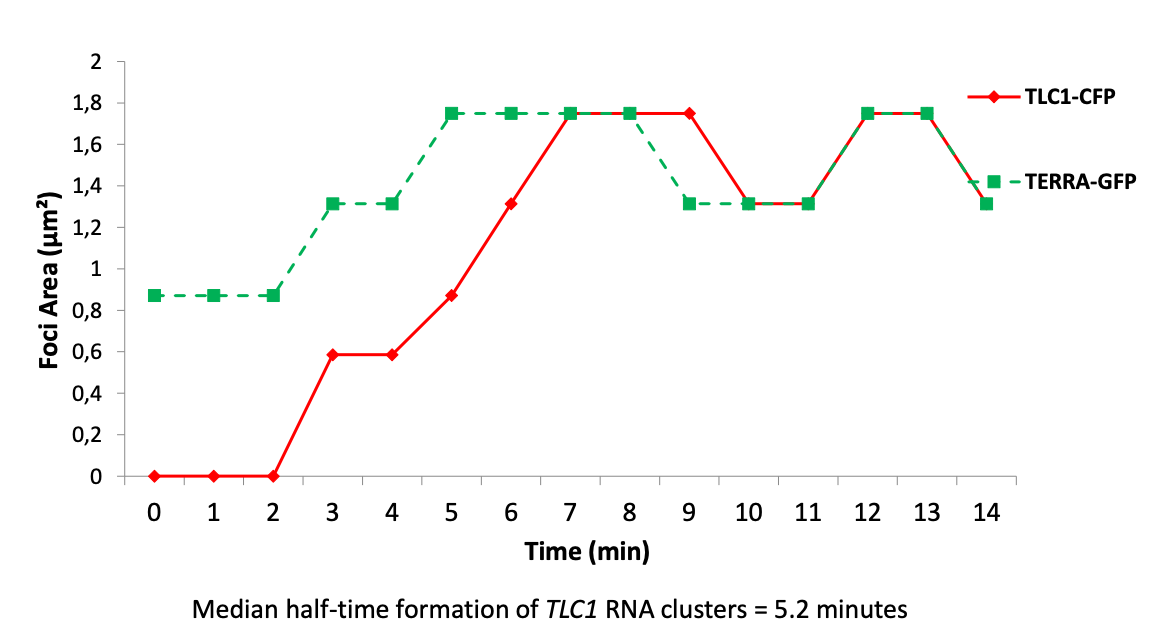
\includegraphics[width=0.5\textwidth]{../_resources/Screen_Shot_2022-12-17_at_11-03-53.png}
\caption{Screen Shot 2022-12-17 at 11-03-53.png}
\end{figure}

Tag simultaneously Tel6R-TERRA and TLC1: by increasing the number of
experiments, it was possible to observe TLC1. The intensity of the
transcript increased over time and co-localized with TERRA (yellow
signal). It was proposed that TERRA foci could act as scaffold for
telomerase clustering.

Generate a system to visualize Tel6R-TERRA, TLC1 and the telomere of
origin for TERRA. Colocalization events between \emph{TLC1} RNA and
telomere 6R, telomerase preferentially localizes at telomeres expressing
TERRA.  If telomeres are short enough, we observe a clustering of
TERRA-TLC1, which promotes telomerase activity.

\begin{figure}
\centering
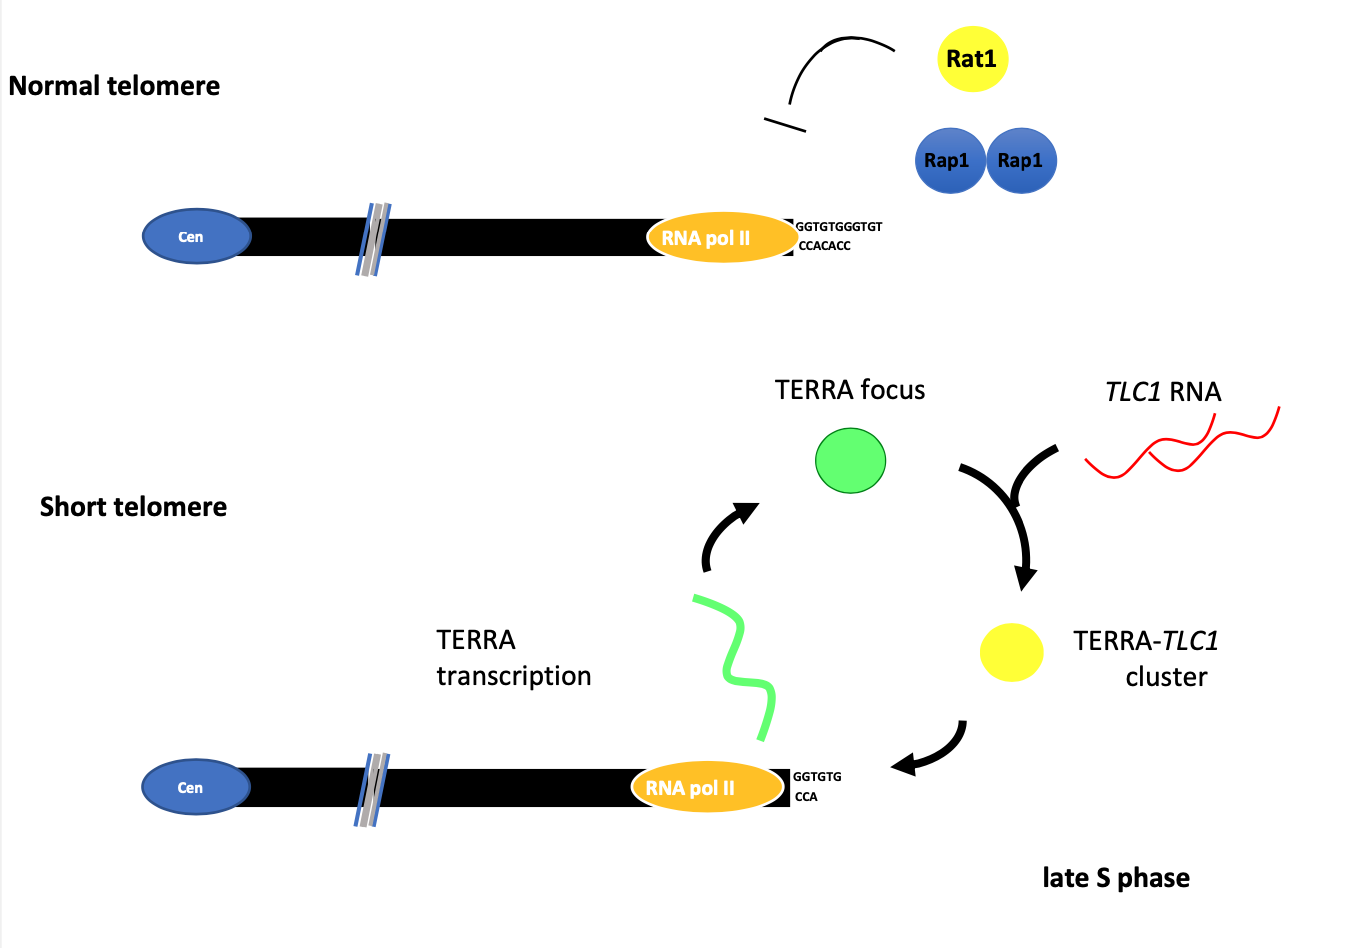
\includegraphics[width=0.5\textwidth]{../_resources/Screen_Shot_2022-12-17_at_11-08-23.png}
\caption{Proposed model for TERRA action at yeast telomeres}
\end{figure}

Proposed model for TERRA action at yeast telomeres

The integration of MS2 sequences at subtelomere 15q in cancer cells can
be performed using the CRISPR/cas9 system. Deplete TERRA from a single
telomere, difficult task as the sequence is identical or almost. DNA
damage response was detected, suggesting that it has both telomeric and
non-telomeric function.

\hypertarget{cusanelli-lab-projects}{%
\subsection{Cusanelli Lab projects}\label{cusanelli-lab-projects}}

Projects ongoing in the lab:

\begin{enumerate}
\def\labelenumi{\arabic{enumi}.}
\tightlist
\item
  Deciphering the function of TERRA in the regulation of telomerase.
  Study of TERRA localization at telomeres during telomere elongation:
  telomerase activity associates with decreased telomeric localization
  of TERRA. Less TERRA-TR are present at telomeres during telomerase
  activity.
\end{enumerate}

TERRA transcripts may interfere with the recruitment of telomerase to
telomeres → inhibitor of telomerase as long as it is on telomeres.
Indeed, TERRA depletion results in increased TR foci formation and TR
localization at telomeres.

\begin{enumerate}
\def\labelenumi{\arabic{enumi}.}
\tightlist
\item
  Mechanisms of TERRA biogenesis: how is pol II dealing with telomeric
  repeats? How is polyadenylation regulated? Polyadenylation occurs in a
  telomeric specific manner.
\item
  Investigating the function of TERRA in ALT induction: depletion of
  ASF1 histone chaperone results in the initiation of the ALT phenotype
  and TERRA localization at telomeres → early stage of activation
\item
  TERRA biology in C. elegans: studied TERRA expression in telomerase
  negative strain, in ALT strains and studied TERRA dynamics using the
  MS2 system
\item
  Investigating the function of TERRA in the cytoplasm
\end{enumerate}

